\chapter{Server}
\label{ch:server}

\author{Nico Kratky}
%
A server is a computer program that supplies clients with services. The term \textit{server} often refers to the machine on which the program is running on. In this project the server has to accomplish several tasks. It has to read data from the sensor that is used, and distribute this data to clients. To do this it also has to manage clients and incoming connection requests.

\section{Raspberry Pi 3 Model B}

The Raspberry Pi is a small single-board computer, developed by the Raspberry Pi Foundation \autocite{RasPi}. Originally it was created to teach children how to use computers and more importantly, how to program them. The biggest advantage of these mini-computers is the variety of extension possibilities. These extensions are so-called HAT's (Hardware Attached on Top) or Shields (which is a term that is more often used when talking about Arduinos). They are connected by using the on-board General-purpose input/output (GPIO) pins. They mostly provide additional hardware to extend the application possibilities and to achieve the desired goal. Further advantages are its relatively small footprint, low cost and wide-variety of available Linux distributions. Having these advantages was the decisive factor for choosing the Raspberry Pi. In this project the latest available version, which is the Raspberry Pi 3 Model B, was used. Specifications of this computer are listed in table \vref{tab:raspispec}.

\begin{table}[h]
    \centering
    \begin{tabularx}{\linewidth}{| l | X |}
    \hline
    \textbf{SoC} & Broadcom BCM2837 \\ \hline
    \textbf{CPU} & 4x ARM Cortex-A53, 1.2GHz \\ \hline
    \textbf{GPU} & Broadcom VideoCore IV \\ \hline
    \textbf{RAM} & 1GB LPDDR2 (900MHz) \\ \hline
    \textbf{Networking} & 10/100 Ethernet, 2.4GHz 802.11n wireless \\ \hline
    \textbf{Bluetooth} & Bluetooth 4.1 Classic, Bluetooth LE \\ \hline
    \textbf{Storage} & microSD \\ \hline
    \textbf{GPIO} & 40-pin header, populated \\ \hline
    \textbf{Ports} & HDMI, 3.5 analogue audio-video jack, 4x USB 2.0, Ethernet, Camera Serial Interface (CSI), Display Serial Interface (DSI) \\ \hline
    \end{tabularx}
    \caption{Raspberry Pi 3 Model B specifications}
    \label{tab:raspispec}
\end{table}

\begin{figure}[H]
	\centering
	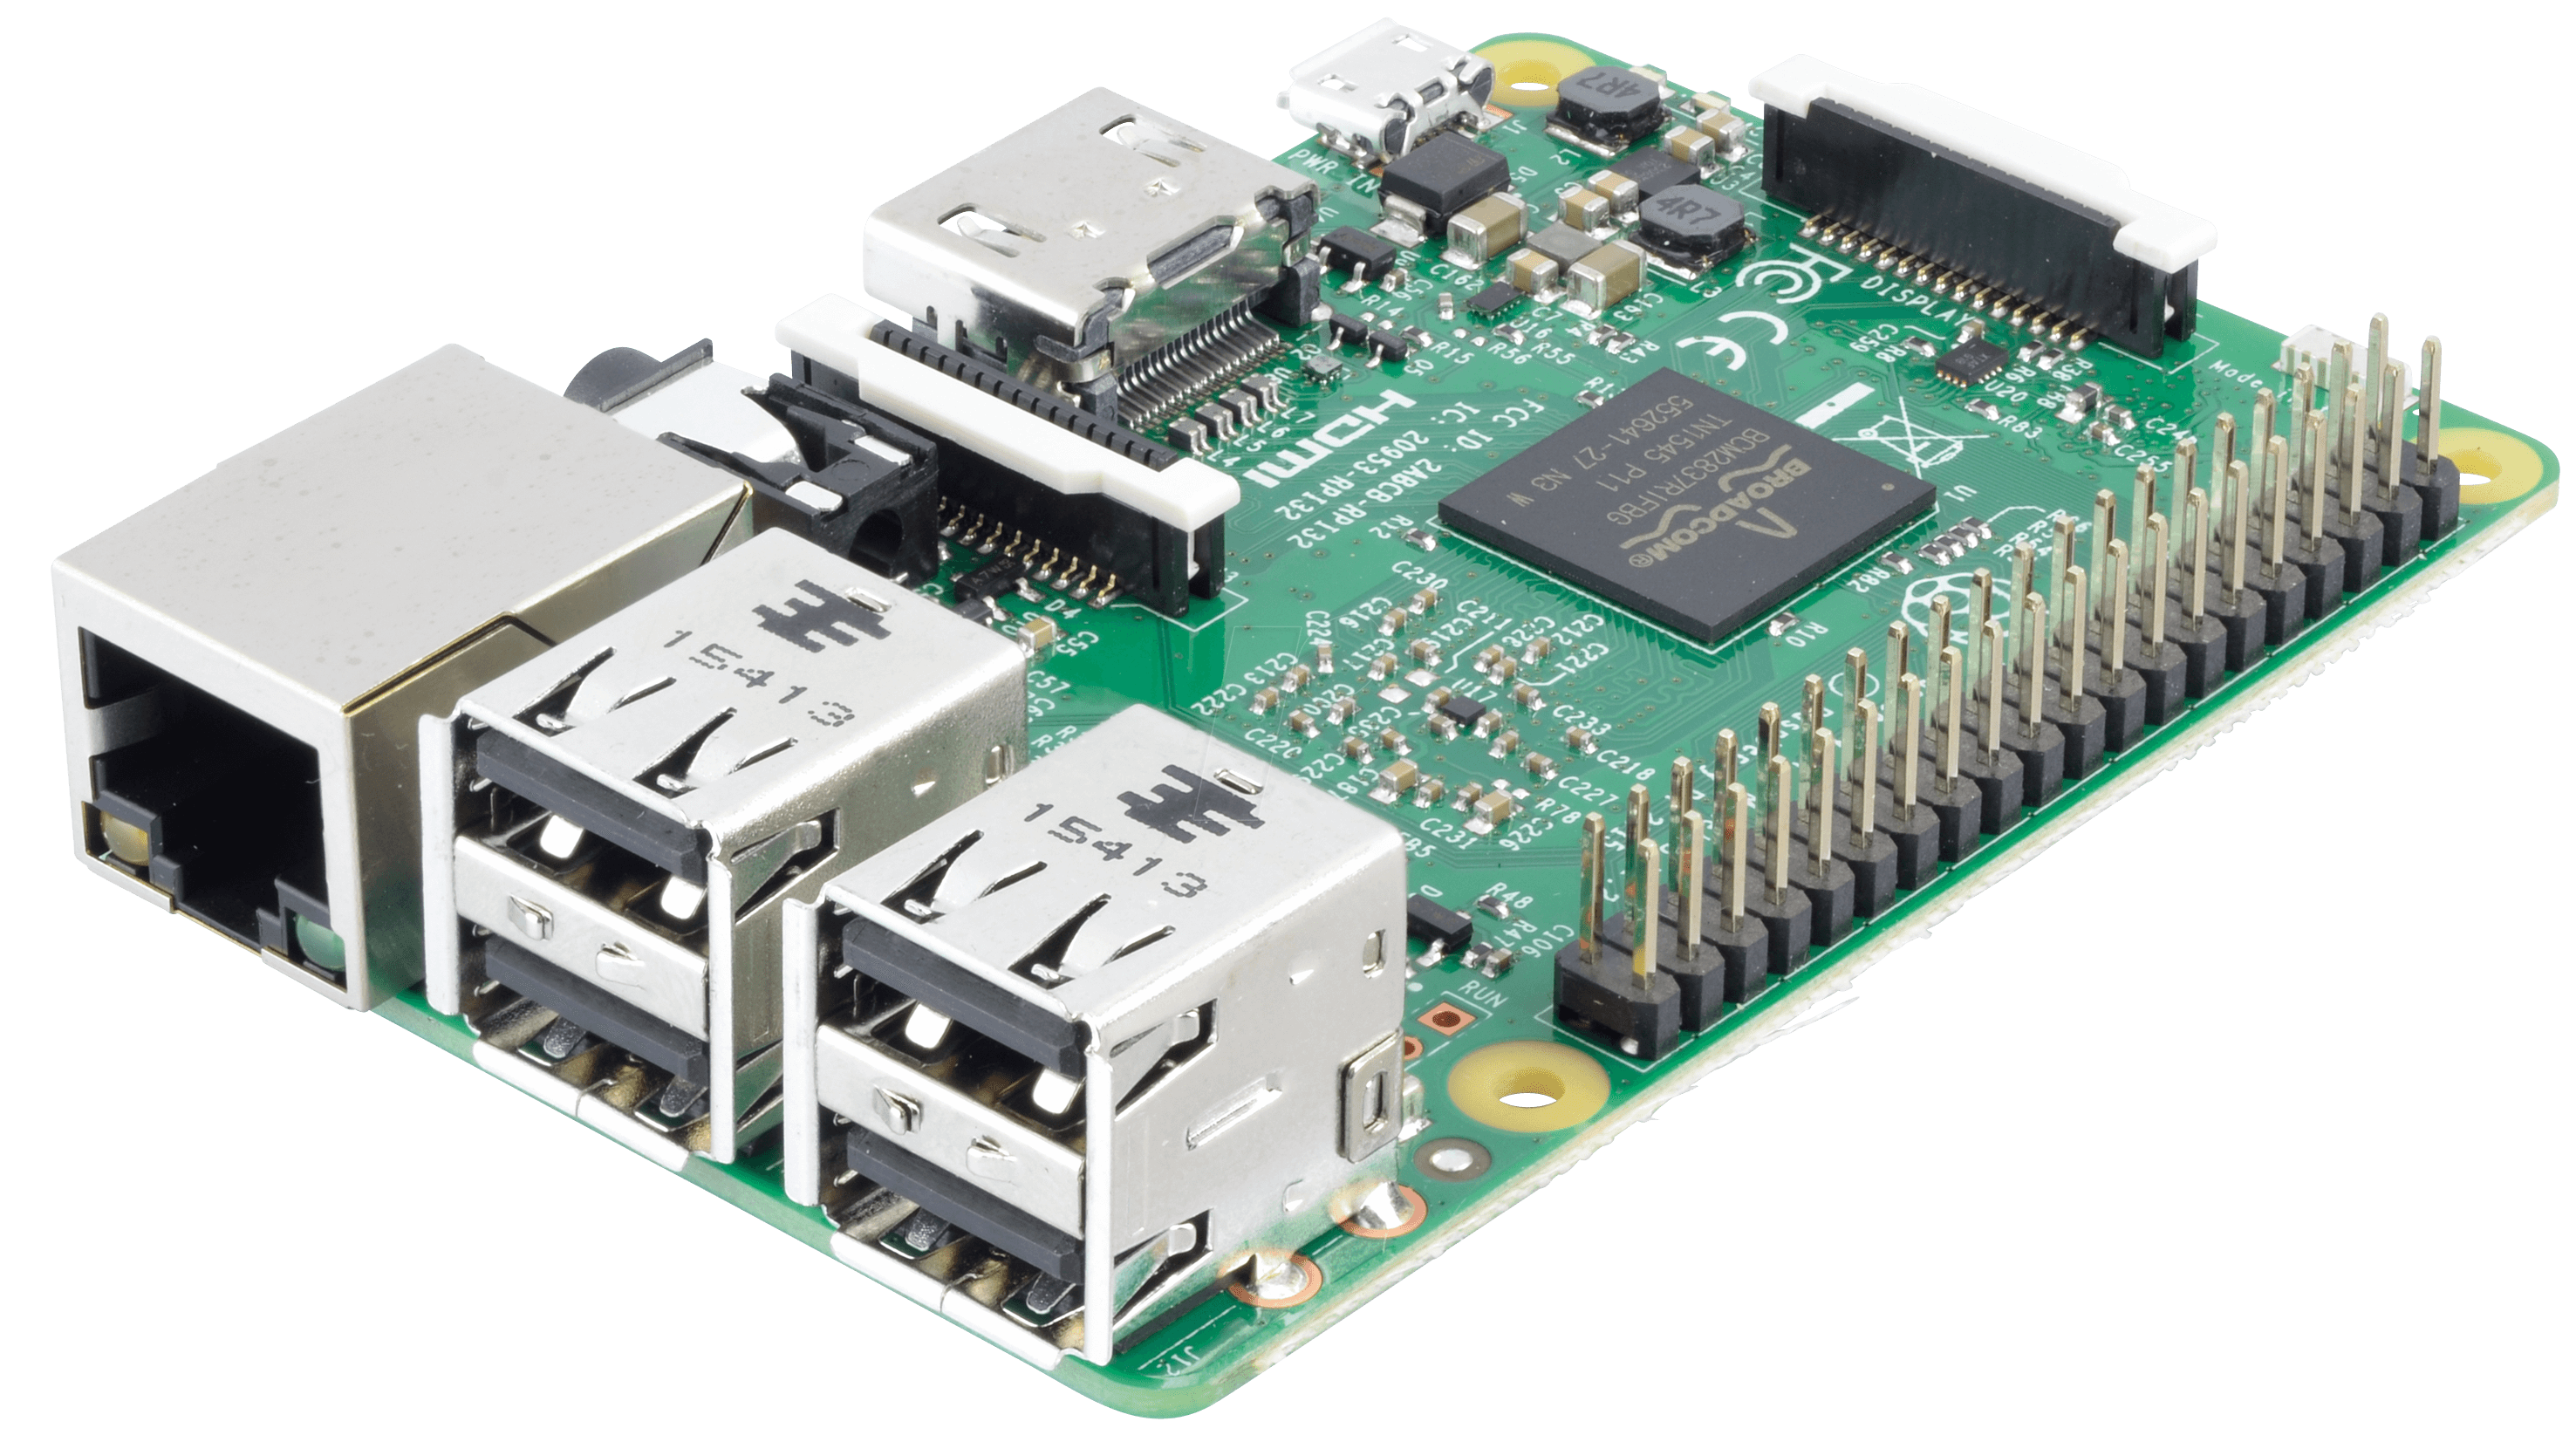
\includegraphics[width=10cm,keepaspectratio]{raspberrypi3b}
	\caption[Raspberry Pi 3 Model B]{Raspberry Pi 3 Model B \autocite{img:raspi}}
	\label{fig:raspberrypi3b}
\end{figure}

\section{Raspberry Pi SenseHAT}

The SenseHAT was made especially for the Astro Pi mission, where students could create and code projects, which were then run on the International Space Station by astronaut Tim Peake \autocite{AstroPiMission}. This board was chosen because it offers a wide variety of sensors and therefore offers many possibilities in terms of testing GRAMOC. Figure \vref{fig:sensehat} shows a SenseHAT that is not attached to a Raspberry Pi.

The Raspberry Pi Sense HAT includes following sensors and inputs/outputs \autocite{SenseHAT}:

\begin{minipage}{\textwidth}
\begin{itemize}
	\item ST LSM9DS1 Inertial measurement sensor
		\begin{itemize}
			\item 3D accelerometer
			\item 3D gyroscope
			\item 3D magnetometer
		\end{itemize}
	\item ST LPS25H barometric pressure and temperature sensor
	\item ST HTS221 relative humidity and temperature sensor
	\item Alps SKRHABE010 5-button mini-joystick
	\item 8x8 RGB LED matrix
\end{itemize}
\end{minipage}

Although GRAMOCs main task is to charactarise steel belts using a magnetometer, a Raspberry Pi SenseHAT add-on board was used to get sensor data. It was dicided to use the now available accelerometer to perform measurements because it is easier to control the sensor data than by using the magnetometer. Different sensor values can be generated by simply moving around the Raspberry Pi with the attached SenseHAT.

\begin{figure}[H]
	\centering
	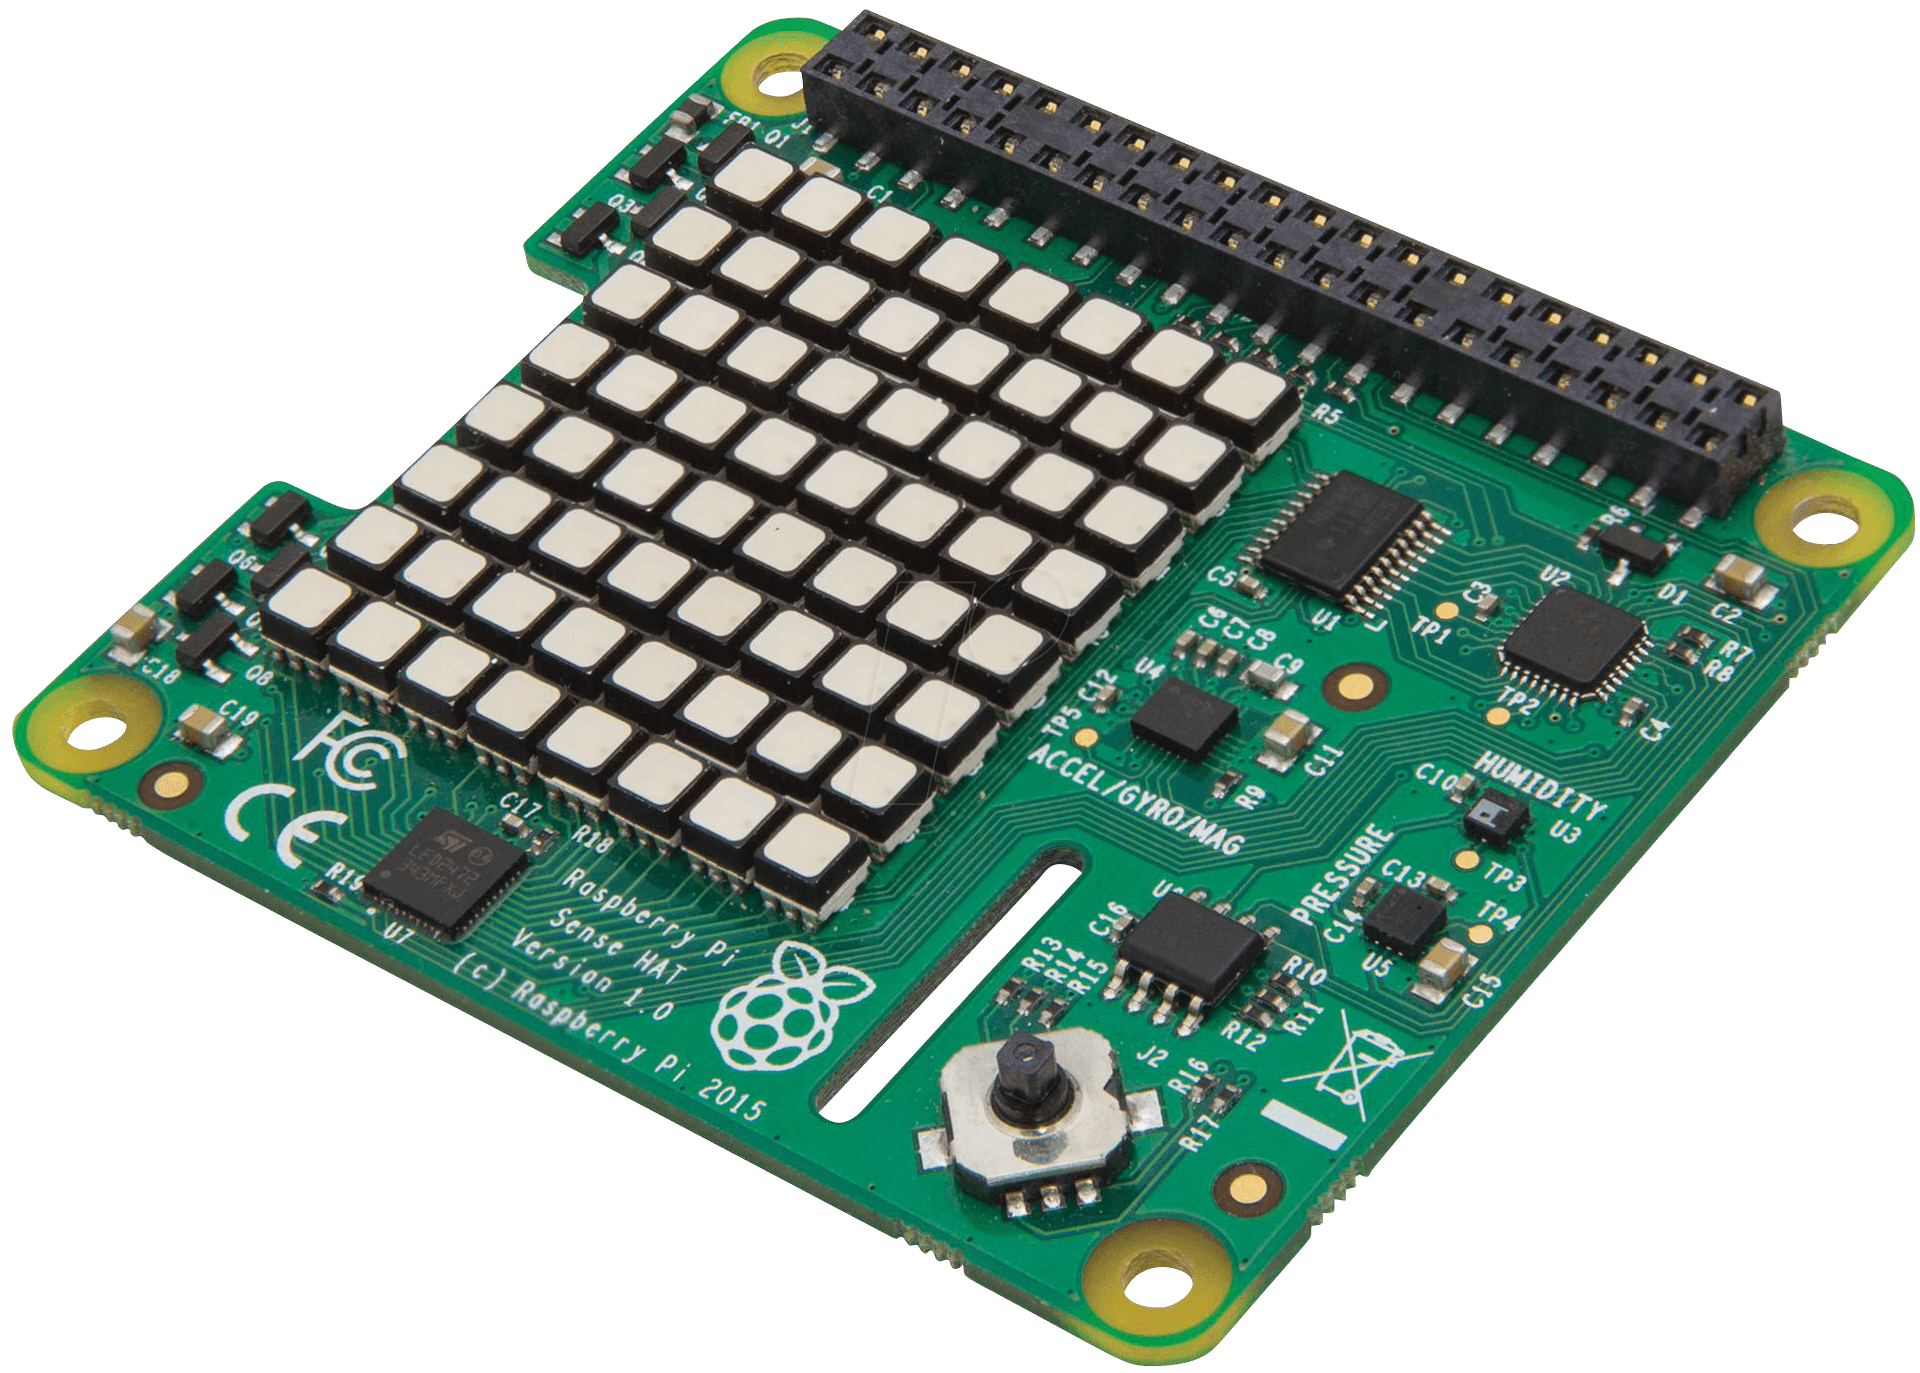
\includegraphics[width=8cm,keepaspectratio]{sensehat}
	\caption[Raspberry Pi SenseHAT]{Raspberry Pi SenseHAT \autocite{img:sensehat}}
	\label{fig:sensehat}
\end{figure}

\section{Implementation}

The server program of GRAMOC is completely written in Python. This allows for great compatibility as Python comes preinstalled on many systems.

\subsection{Programming Language}

Python is a simple yet powerful modern programming language and supports both procedure-oriented as well as object-oriented programming. It was developed by Guido van Rossum at Centrum Wiskunde \& Informatica (CWI) in the Netherlands in 1989 and first released in 1991 \autocite{HistoryOfPython}. It was meant to be a successor to the ABC programming language. Python is a high-level language and therefore includes features such as automatic memory management.

Python is currently available in version 3.6.2. Nevertheless version 2.7 is still available as the Python Software Foundation announced that it will be supportet until 2020, effectivly making it an Long-term support version. Despite that, Python 3.6.2 was chosen for GRAMOC as the Foundation also encourages users to use the newest version if possible. Another reason for choosing the newer version is that GRAMOC does not have to be backwards compatible to any existing software.

\section{Program Flow}

As depicted in figure \vref{fig:server-program-flow}, the server starts accepting new connections right after is has started. It then performs the handshake that is required by GSDEP (further explained in \vref{sec:networking_data-flow}). If this handshake is performed without errors, the server starts listening for data from this now connected client on a separate thread. While this thread is running it receives one message and checks if it is a command (see \vref{sec:networking_command}). If it is, the message is interpreted and the appropriate function is executed. This thread is kept alive until the client disconnects or the server is shutdown by the user.

\begin{figure}[H]
	\centering
	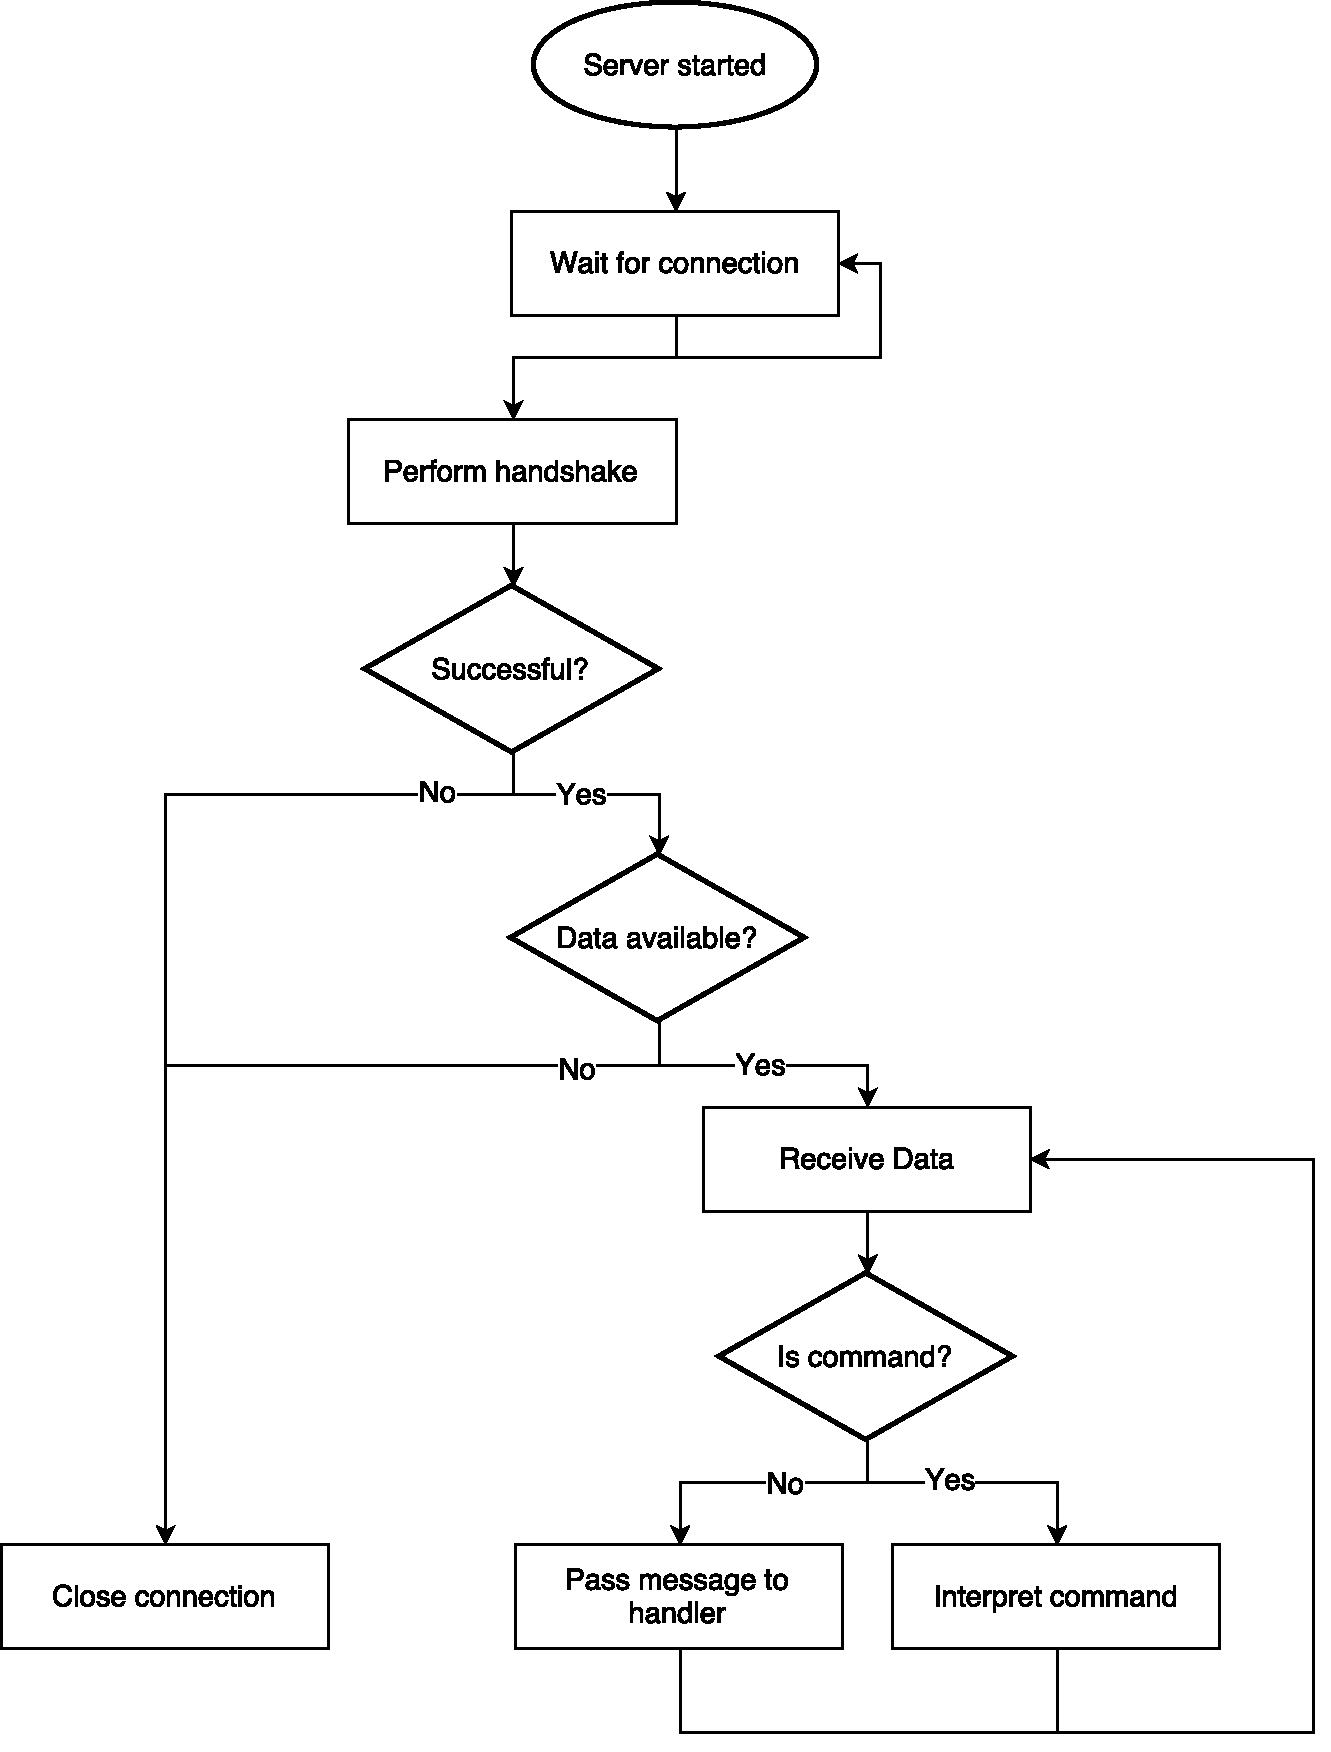
\includegraphics[width=13cm,keepaspectratio]{server-task}
	\caption{Flowchart of server program showing the procedure}
	\label{fig:server-program-flow}
\end{figure}
